\documentclass{beamer}

\usepackage{babel}
\usepackage{tikz}
%\usetheme{boxes}
\usepackage[utf8]{inputenc}
\usepackage{amsmath}
\usepackage{amsthm}
\usepackage{hyperref}
\usepackage{natbib}
\usepackage{tikz}
\usepackage{xcolor}
\usepackage[absolute,overlay]{textpos}
\bibliographystyle{plainnat}
\usecolortheme{crane}

\definecolor{orange}{RGB}{232, 86, 15}
\definecolor{blue}{RGB}{14, 159, 232}
\definecolor{blueblue}{RGB}{50, 90, 160}
\definecolor{yellow}{RGB}{232, 187, 14} 
\definecolor{red}{RGB}{232, 14, 59}
\newtheorem{deff}{Definición}
%Information to be included in the title page:
\institute[]{}

\setbeamercolor{title}{bg=blueblue, fg=white}
\setbeamercolor{subttile}{bg=blueblue, fg=white}
\setbeamercolor{frametitle}{bg=blueblue, fg=white}
\setbeamercolor{block title}{bg=blue, fg=white}
\setbeamercolor{block title alerted}{bg=red, fg=white}
\setbeamercolor{block title example}{bg=yellow, fg=white}
\setbeamercolor{footline}{bg=gray, fg=white}
\beamertemplatenavigationsymbolsempty

	
\newcommand{\indep}{\perp \!\!\! \perp}

\newcommand\blfootnote[1]{%
  \begingroup
  \renewcommand\thefootnote{}\footnote{#1}%
  \addtocounter{footnote}{-1}%
  \endgroup
}


\newcommand\overalert[2]{
	 \only<#1>{
\begin{textblock*}{\textwidth}(.35\textwidth,0.25\textheight)
    \begin{beamercolorbox}[wd=.5\textwidth,center,sep=0.3cm]{block title alerted}
	    #2
    \end{beamercolorbox}
\end{textblock*}
}
}

\newcommand\overexample[2]{
	 \only<#1>{
\begin{textblock*}{\textwidth}(.35\textwidth,0.25\textheight)
    \begin{beamercolorbox}[wd=.5\textwidth,center,sep=0.3cm]{block title example}
	    #2
    \end{beamercolorbox}
\end{textblock*}
}
}


\newcommand\overeblock[2]{
	 \only<#1>{
\begin{textblock*}{\textwidth}(.35\textwidth,0.25\textheight)
    \begin{beamercolorbox}[wd=.5\textwidth,center,sep=0.3cm]{block title}
	    #2
    \end{beamercolorbox}
\end{textblock*}
}
}

\title{The (Casual) Causality Course \\ Introduction, some notations and fundamentals}
\author{Gherardo Varando}
\date{IPL \\ 02 May 2023}
\begin{document}

\begin{frame}
	\titlepage
\end{frame}

\begin{frame}{The course}

	\begin{itemize}
		\item \textbf{When:} Tuesday and Thursday from 10:30 to 13:00 for the next 4 weeks
		\item \textbf{Where:} In person IPL hall and (limited) virtual at zoom link
			              \url{https://uv-es.zoom.us/j/94222318081?pwd=NkNGOForRDYrNEtuUHR2cGFmQWN6Zz09}
		\item \textbf{Who:}  Gherardo Varando (gherardo.varando@uv.es) and 
			Emiliano Díaz (emiliano.diaz@uv.es)
		\item \textbf{Material} available on github \url{https://github.com/IPL-UV/casual_causality_course} if you are in the IPL you should have access to the private repo, otherwise write me an email with your github email and username and I will grant you access. 
	\end{itemize}

\end{frame}

\begin{frame}{Content}
	\begin{itemize}
		\item[Week 1] \textbf{Introduction and notations}
			\begin{itemize}
				\item[Tue 02] Course introduction and first concepts 

		%statistical vs causal model, BN/DAG, SEM, interventions and counterfactuals 

	\item[Thur 04] Causal frameworks and framing causal problems 
			\end{itemize}
		\item[Week 2] \textbf{Causal Discovery} 
			\begin{itemize}
		            \item[Tue 09] Classical approaches 
			    \item<2->[Wed 10?] \textcolor{red}{Practical session on causal discovery?}
		            \item[Thur 11] Continuous optimization methods and NN parametrizations
			\end{itemize}
		\item[Week 3] \textbf{Causal Inference} 
			\begin{itemize}
		            \item[Tue 16] Causal effect estimation and possible biases  
		            \item[Thur 18] Machine learning methods for causal effect estimation
			\end{itemize}
		\item[Week 4] \textbf{Applications} 
			\begin{itemize}
                           \item[Tue 23]  
                           \item[Thur 25] 
			\end{itemize}

	\end{itemize}
\end{frame}


\begin{frame}{Statistical Models: a very short story}
	\begin{itemize}
		\item A mathematical model of the data generating process
		\item A description of the probability of data  
		\item A collection of statistical assumptions 
		\item Allows us to compute probabilities of events 
	\end{itemize}
	\begin{block}{Definition}
		Formally we can define a statistical model as a pair $(\mathcal{S}, \mathcal{P})$
		where
		\begin{itemize}
			\item $\mathcal{S}$ is a sample space, 
				formally $\mathcal{S} = (\Omega, \mathcal{F})$ with $\mathcal{F}$ a $\sigma$-algebra on $\Omega$ a set 
			\item $\mathcal{P}$ is a collection of probability distributions on $\mathcal{S}$ 
		\end{itemize}
	\end{block}
	Usually $\mathcal{P}$ is indexed by some finite-dimensional parameter $\theta$, in that case the model is said to be \textbf{parametric}, if instead the parameter is infinite dimensional (or there is no parameter) the model is said to be \textbf{non-parametric}.
	\blfootnote{\citep{wasserman2004all}}
\end{frame}

\begin{frame}{Inference and statistical problems}
	\begin{itemize}
		\item<1-> modelling the data     
			\vspace{0.3cm}
		\item<2-> prediction or forecasting 
			\vspace{0.3cm}
		\item<3-> queries on parameter(s)  
			\vspace{0.3cm}
	        \item<4-> decision making  
			\vspace{0.3cm}
		\item<5-> model selection 
	\end{itemize}
	\onslide<6->{
		\begin{example}{}
                       image classification, weather forecasting, stock price prediction, 
		       crop yield prediction,  crop detection, cloud detection, gap-filling
		\end{example}
	}
\end{frame}


\begin{frame}{Regression models}
	\begin{columns}
		\begin{column}{0.5\textwidth}
    Given data $(X_i, Y_i)$ 
	\begin{itemize}
		\item<1-> find best function that approximate $Y = f(X)$
		\item<2->  define a statistical model for $P(Y|X)$, 
			e.g. if consider an additive noise model $Y = f(X) + \varepsilon$ 
		\item<3-> linear case  $Y = \sum \beta_i X_i + \beta_0 + \varepsilon$ 
			we can do inference on the parameters $\beta_i$: confidence intervals, hypothesis testing
		\item<4-> non-parametric approaches, for example kernel methods 
		\item<4-> non-additive noise models, $Y = f(X, \varepsilon)$ 
	\end{itemize}
		\end{column}
		\begin{column}{0.5\textwidth}
	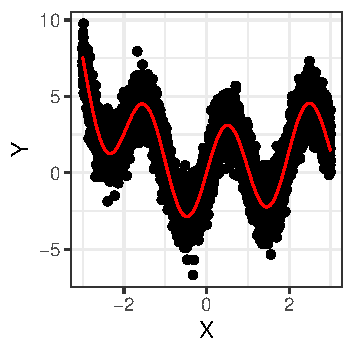
\includegraphics{images/regression}
		\end{column}
		\end{columns}

		\overexample{5}{How we can expand a regression model to obtain a full statistical model for the joint probability $P(X,Y)$?} 

\end{frame}

\begin{frame}{Bayesian Networks}

	\begin{block}{Definition}
              A Bayesian Network (BN) over random variables $X_1, X_2, \ldots, X_p$ 
		is a pair $(G, P)$ where
		\begin{itemize}
			\item $G$ is a DAG over $p$ nodes (indexed as the r.vs)  
			\item $P$ is a joint probability over $X_1, \ldots, X_p$ such that 
				$P = \prod_{i=1}^p P(X_i| X_{pa(i)} )$
		\end{itemize}
	\end{block}

	\begin{itemize}
		\item BNs are an example of probabilistic graphical models 
		\item  define statistical models 
		\item<2-> for categorical r.v.s $P(X_i| X_{pa(i)})$ can be represented 
			with conditional probability tables (CPTs)
		\item<3-> for Gaussian r.v.s (and linear relationships), it is sufficient to specify a 
			set of (linear) regressions for each node over its parents and the variance
			of the residuals
	\end{itemize}
	\blfootnote{\citep{lauritzen1996graphical, koller2009probabilistic, 
	maathuis2018handbook}}
	\overeblock{4}{\citep{wasserman2004all} and others think that the term Bayesian Network 
	is misleading and poor terminology since BN do not have anything to do with Bayesian methods} 
\end{frame}

\begin{frame}
	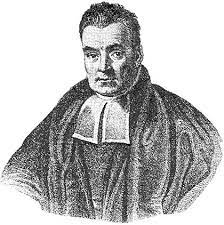
\includegraphics{images/bayes}
	\overexample{2}{Thomas Bayes (c. 1701 – 7 April 1761) was an English statistician, 
	philosopher and Presbyterian minister who is known for formulating a 
	specific case of the theorem that bears his name: Bayes' theorem.}
\end{frame}

\begin{frame}

\begin{columns}
	\begin{column}{0.5\textwidth}
		\begin{itemize}
			\item<2-> 
				\begin{enumerate}
					\item parents $pa(i)$
					\item children $ch(i)$
					\item descendants $de(i)$
					\item non-descendants $nde(i)$
					\item ancestrors $an(i)$
				\end{enumerate}
			\item<3-> {v-structures, immoralities}
			\item<4-> moral graph $G^m$ 

			\item<5-> topological order   

		\end{itemize}
	\overexample{7}{can you write the factorization of the joint probability associated with this graph?}

	\end{column}
	\begin{column}{0.5\textwidth}
		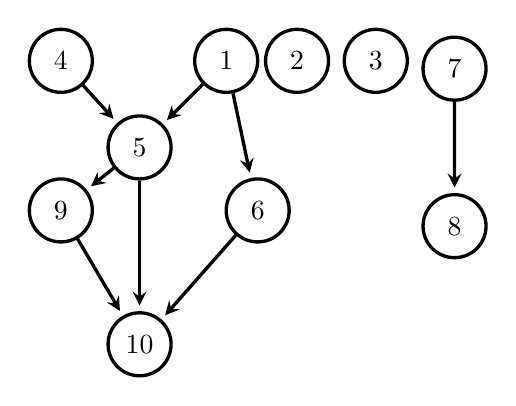
\begin{tikzpicture}[scale=5, 
       node/.style={circle,inner sep=1mm,minimum size=0.8cm,draw,
      very thick,black,fill=white,text=black},
        nondirectional/.style={very thick,black},
        unidirectional/.style={nondirectional,shorten >=2pt,-stealth},
        bidirectional/.style={unidirectional,bend right=10}]

	\node [node] (v1) at (0.420000, 0.720000)       {1};
        \node [node] (v2) at (0.60000, 0.720000)        {2};
        \node [node] (v3) at (0.80000, 0.720000)        {3};
        \node [node] (v4) at (0.00000, 0.720000)        {4};
        \node [node] (v5) at (0.200000, 0.500000)       {5};
        \node [node] (v6) at (0.500000, 0.340000)       {6};
        \node [node] (v7) at (1.000000, 0.700000)       {7};
        \node [node] (v8) at (1.000000, 0.300000)       {8};
        \node [node] (v9) at (0.00000, 0.340000)        {9};
	\node [node] (v10) at (0.200000, 0.000000)      {10};

        \path [unidirectional] (v1) edge (v5);
        \path [unidirectional] (v4) edge (v5);
        \path [unidirectional] (v5) edge (v9);
        \path [unidirectional] (v5) edge (v10);
        \path [unidirectional] (v1) edge (v6);
        \path [unidirectional] (v6) edge (v10);
        \path [unidirectional] (v7) edge (v8);
        \path [unidirectional] (v9) edge (v10);
\end{tikzpicture}
	
	\end{column}
\end{columns}

\end{frame}

\begin{frame}
 \begin{itemize}
	 \item<1-> BNs are statistical models  
	 \item<2-> statistical models are "collection of statistical assumptions" 
         \item<3-> which are the assumptions associated with a given BN $(G, P)$?
 \end{itemize}
	\onslide<4->\begin{block}{BN/DAG and conditional independences}
		The following statements are equivalent:
		\begin{itemize}
			\item $(G, P)$ is a BN, that is $P$ factorize recursively wrt the DAG $G$ 
			\item $P$ satisfies the \emph{local Markov property} wrt $G$, that is 
				$X_i \indep X_{nd(i)} |  X_{pa(i)}$ 
			\item $P$ satisfies the \emph{global Markov property} wrt $G$, that is
				$X_A \indep X_B | X_D$  whenever $A$ and $B$ are d-separated 
				by $D$ in DAG $G$ ($A$ and $B$ are separated by $D$ in $G_{an(A \cup B \cup D)}^m$)
		\end{itemize}
	\end{block}
	\overeblock{5}{\textbf{ takeaway \\ BN/DAG are graphical ways to encode conditional independence statements}} 
\end{frame}

\begin{frame}
	\begin{columns}
		\begin{column}{0.5\textwidth}
			\begin{itemize}
			\item<1-> d-separation, equivalent to separation in the moral graph of 
				the ancestors of involved vertices 
			\item<2-> equivalently $i$ and $j$ are d-separated by $D$ if 
				there exists no undirected path $u$
					between $i$ and $j$ such that 
					\begin{enumerate}
						\item every collider in $u$ has 
							a descendants in $D$ 
						\item no other vertex on $u$ is in $D$
					\end{enumerate}
			\end{itemize}
		\overexample{3}{Can you list some d-separations in the graph? some are easy ...}
		\end{column}
	\begin{column}{0.5\textwidth}
		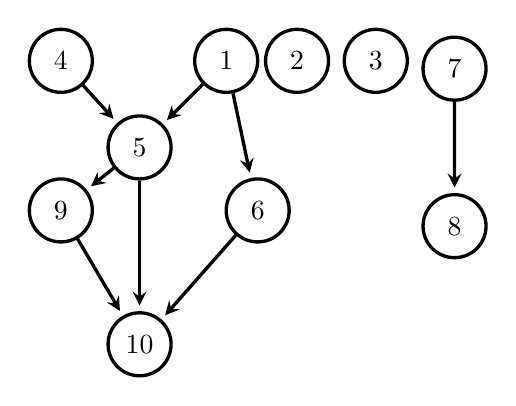
\begin{tikzpicture}[scale=5, 
       node/.style={circle,inner sep=1mm,minimum size=0.8cm,draw,
      very thick,black,fill=white,text=black},
        nondirectional/.style={very thick,black},
        unidirectional/.style={nondirectional,shorten >=2pt,-stealth},
        bidirectional/.style={unidirectional,bend right=10}]

	\node [node] (v1) at (0.420000, 0.720000)       {1};
        \node [node] (v2) at (0.60000, 0.720000)        {2};
        \node [node] (v3) at (0.80000, 0.720000)        {3};
        \node [node] (v4) at (0.00000, 0.720000)        {4};
        \node [node] (v5) at (0.200000, 0.500000)       {5};
        \node [node] (v6) at (0.500000, 0.340000)       {6};
        \node [node] (v7) at (1.000000, 0.700000)       {7};
        \node [node] (v8) at (1.000000, 0.300000)       {8};
        \node [node] (v9) at (0.00000, 0.340000)        {9};
	\node [node] (v10) at (0.200000, 0.000000)      {10};

        \path [unidirectional] (v1) edge (v5);
        \path [unidirectional] (v4) edge (v5);
        \path [unidirectional] (v5) edge (v9);
        \path [unidirectional] (v5) edge (v10);
        \path [unidirectional] (v1) edge (v6);
        \path [unidirectional] (v6) edge (v10);
        \path [unidirectional] (v7) edge (v8);
        \path [unidirectional] (v9) edge (v10);
\end{tikzpicture}
	
	\end{column}
\end{columns}
\end{frame}


\begin{frame}{Sampling from a BN}

How can we obtain samples from a probability distribution 
associated with a BN? 

	\onslide<2-> \textbf{we can use the topological order to sample efficiently}
	\begin{itemize}
		\item pick a topological order of the nodes in $G$ 
		\item to generate each sample:
	\begin{enumerate}
		\item start by sampling $x_i$ from $P(X_i)$ for each nodes $i$ without parents (there must be at least one) 
		\item follow the topological order and sample from $P(X_i| X_{pa(i)} = x_{pa(i)})$ 
			(since we follow the topological order $x_{pa(i)}$ is already sampled) 
	\end{enumerate}
	\end{itemize}

\end{frame}

\begin{frame}{Other graphical models}
	\begin{itemize}
		\item Markov networks, Markov random fields or undirected graphical models (e.g. Ising models in statistical physics) \citep{koller2009probabilistic, lauritzen1996graphical} 
		\item Model based on event trees such as staged event trees or chain event graphs
			\citep{leonelli23a}
		\item Chain graphs 
		\item restricted Boltzman machines 
	\end{itemize}
	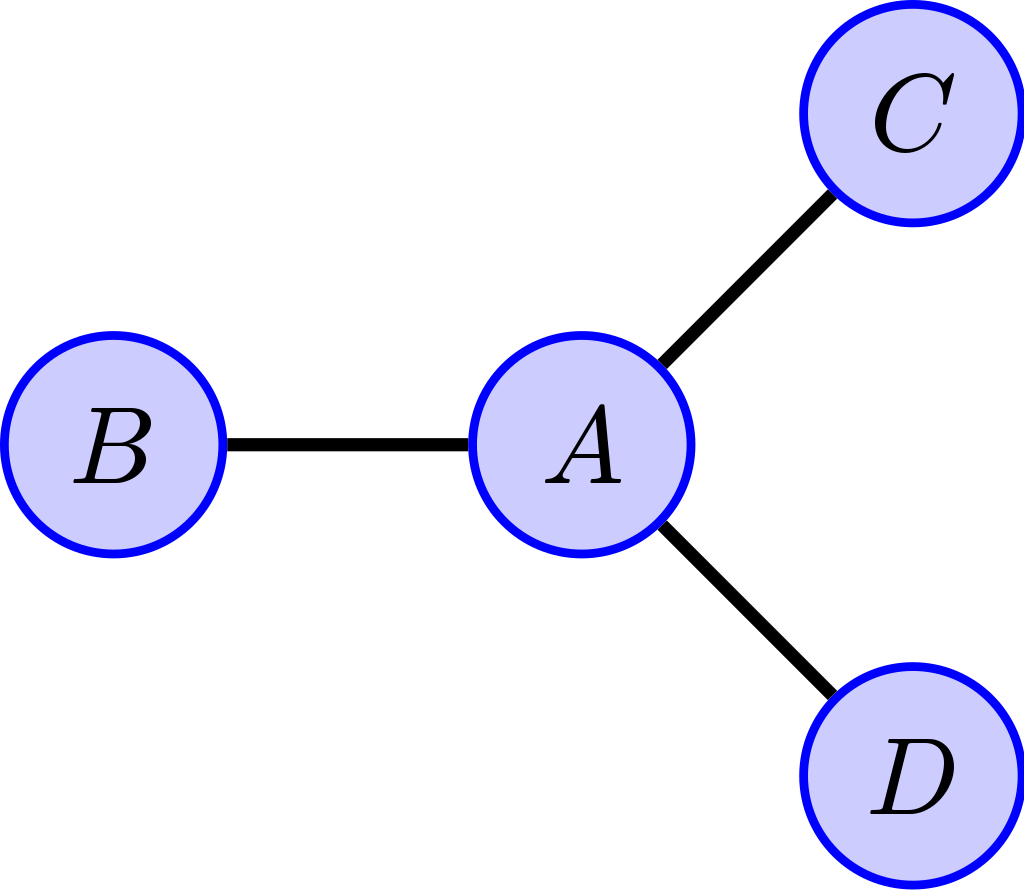
\includegraphics[scale=0.08]{images/undirected}
	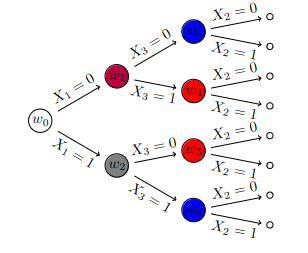
\includegraphics[scale=0.3]{images/tree}
	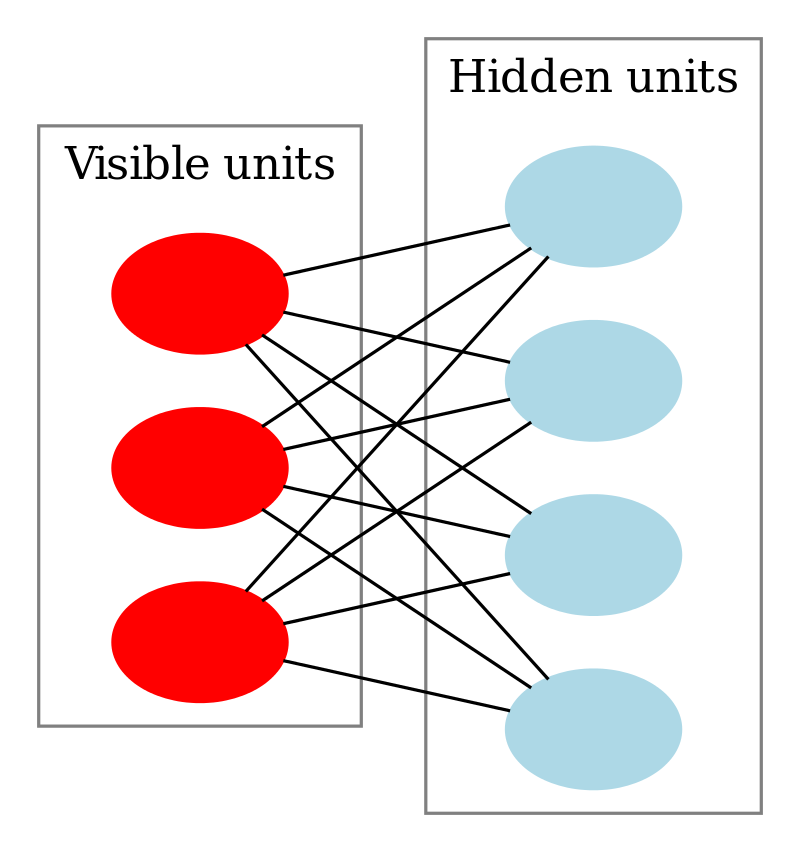
\includegraphics[scale=0.1]{images/restricted}
\end{frame}

\begin{frame}{Causality?} 
	\begin{itemize}
		\item<1-> statistical models (and ML models) represents association in the data 
		\item<2-> stat/ML models are not mechanistic/physical/causal models of the data 
		\item<3-> sometime in the sciences, but also in healthcare, econometrics, \ldots
			we are actually interested in causal questions
		\item<4-> but what is \emph{causality} ? 
	\end{itemize}

\end{frame}

\begin{frame}
	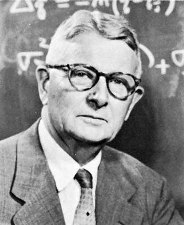
\includegraphics{images/wright}
	\overexample{2}{Sewall Green Wright FRS(For) Honorary FRSE (December 21, 1889 – March 3, 1988) 
	was an American geneticist known for his influential work on evolutionary 
	theory and also for his work on path analysis.
        Path analysis is considered by Judea Pearl to be a direct ancestor
	to the techniques of Causal inference.
	}
\end{frame}



\begin{frame}{(Probabilistic) Causal Models}
	\begin{itemize}
		\item<1-> we consider a probabilistic definition for causality 
		\item<2-> \emph{Roughly speaking, the statement "X causes Y" means that changing the
			value of X will change the distribution of Y} \citep{wasserman2004all} 
		\item<3-> Causal models contain more information than statistical models  
			\citep{peters2017elements}
	\end{itemize}
	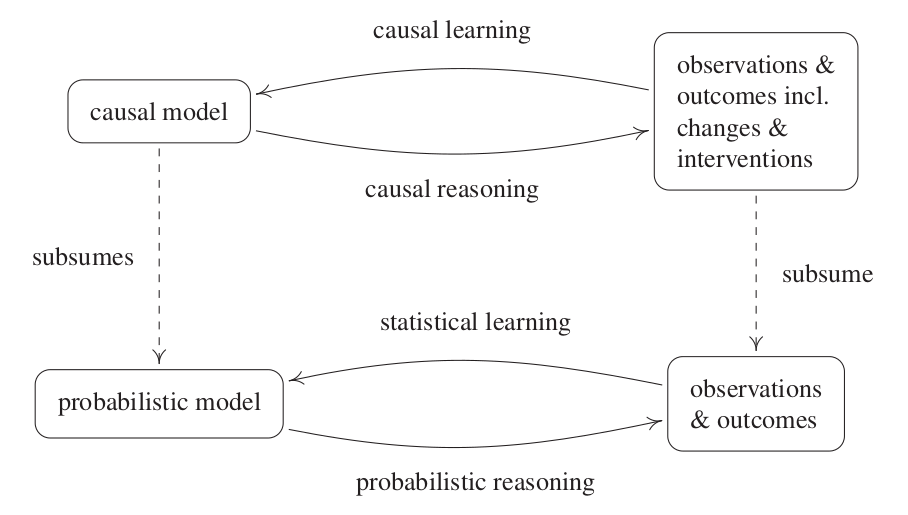
\includegraphics[scale=0.3]{images/causal-diagram}
\end{frame}

\begin{frame}{\emph{correlation does not imply causation}}
	\only<1-1>{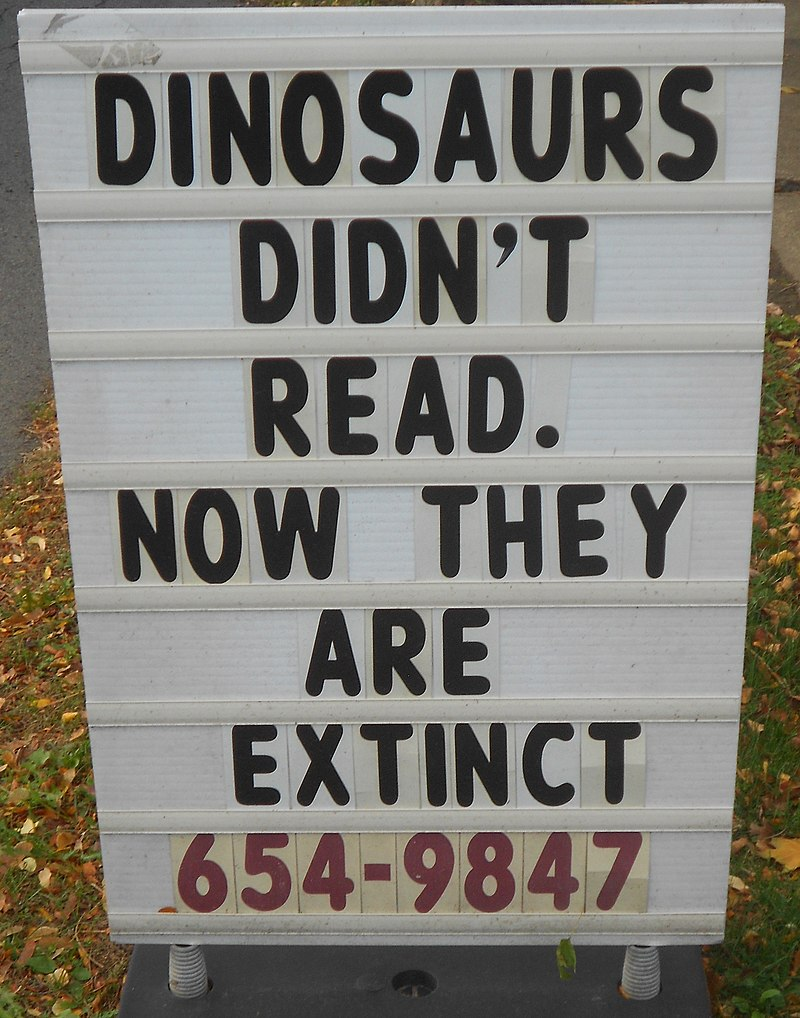
\includegraphics[scale=0.2]{images/dinos}}
	\only<2->{\begin{block}{Reichenbach’s common cause principle\citep{peters2017elements}}
If two random variables $X$ and $Y$ are statistically dependent ($X \not\indep Y$ ), 
		then there exists a third variable
$Z$ that causally influences both. 
		(As a special case, $Z$ may coincide with either $X$ or $Y$.) 
		Furthermore, this variable $Z$ screens $X$ and $Y$ 
		from each other in the sense that given $Z$, 
		they become independent, $X \indep  Y | Z$.
	\end{block}
	In practice other reasons could be:
	\begin{itemize}
		\item<3-> \textbf{time dependence} and thus $X$ and $Y$ appear correlated 
		\item<5-> conditioned on others (\textbf{selection bias}) 
		\item<7-> statistical and finite sample problems 
	\end{itemize}
	\overexample{4}{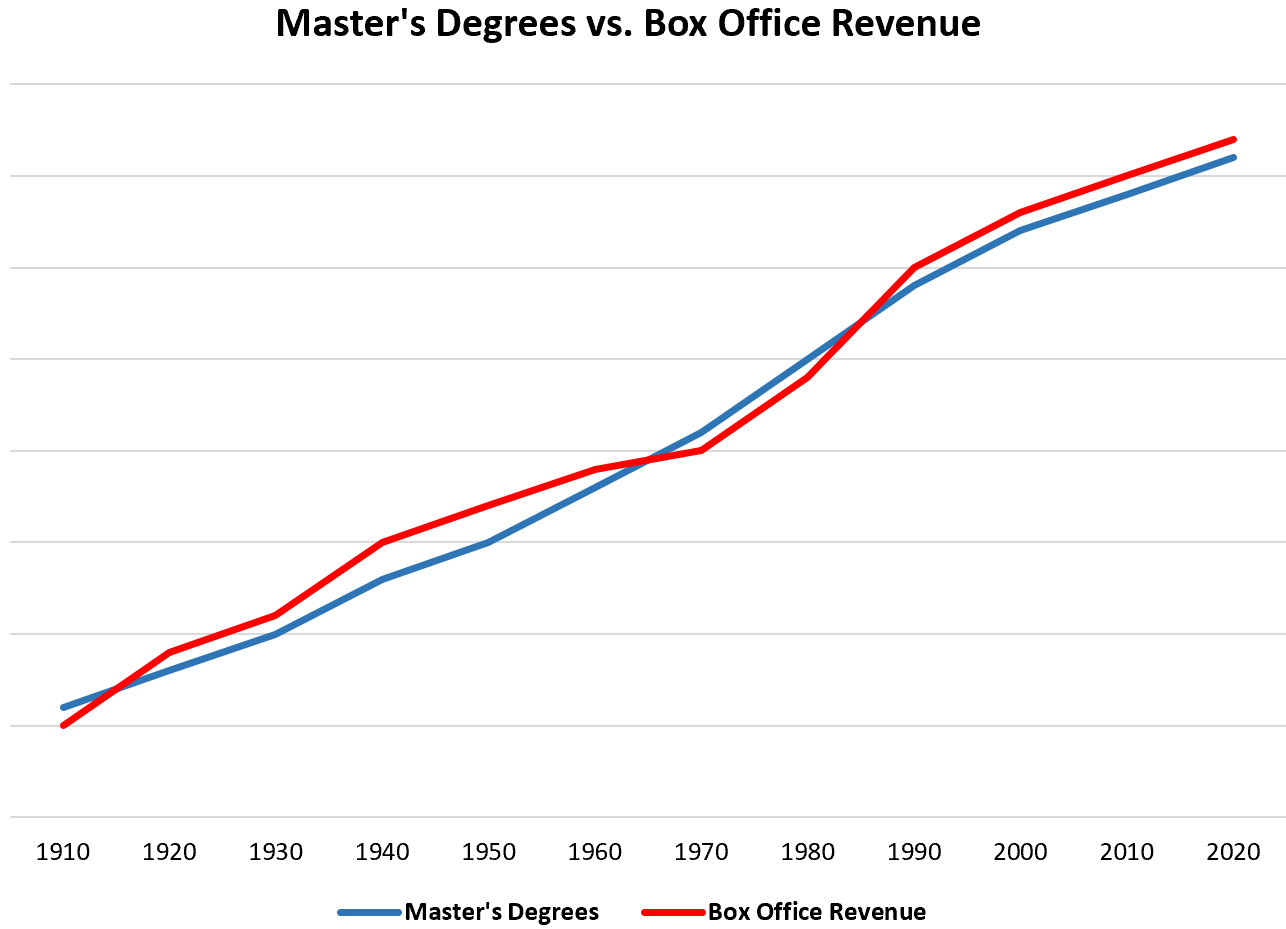
\includegraphics[scale=0.3]{images/corrCause2}}
	\overexample{6}{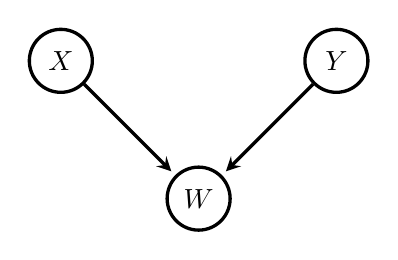
\begin{tikzpicture}[scale=3.5, 
       node/.style={circle,inner sep=1mm,minimum size=0.8cm,draw,
      very thick,black,fill=white,text=black},
        nondirectional/.style={very thick,black},
        unidirectional/.style={nondirectional,shorten >=2pt,-stealth},
        bidirectional/.style={unidirectional,bend right=10}]

	\node [node] (v1) at (-0.5, 0.5)       {$X$};
        \node [node] (v2) at (0.5, 0.5)        {$Y$};
        \node [node] (v3) at (0, 0)        {$W$};

        \path [unidirectional] (v1) edge (v3);
        \path [unidirectional] (v2) edge (v3);
\end{tikzpicture}
}
	}
\end{frame}

\begin{frame}
	\center 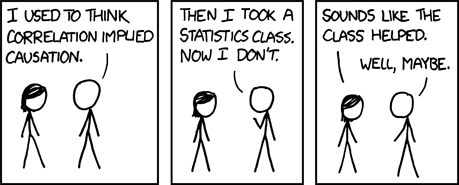
\includegraphics[scale=0.5]{images/correlation}
	\footnote{\url{https://xkcd.com/552}}
\end{frame}

\begin{frame}{Causal models desiderata}
	\begin{itemize}
		\item Represent data, similar to a statistical model 
		\item Model what happen when changes/experiment/interventions  
		\item Reason on and explore the causal relationships 
		\item Represent causal realtionships 
	\end{itemize}
\end{frame}

\begin{frame}{Causal regression models}
      \begin{itemize}
	      \item given a regression model $Y = f(X, \varepsilon)$ 
		      we could interpret this as a causal model 
	      \item in the sense that we immagine the physical/true generating process 
		      to be modeled by this equation 
	      \item<2-> If we make \emph{experiments} by changing the value of $X$ we know that 
		      the associated value for $Y$ is generated accordingly to $f(X, \varepsilon)$ 
      \end{itemize}
\end{frame}

\begin{frame}{Structural Causal Models}
	\begin{block}{Definition \citep{peters2017elements}}
 A SCM over variables $X_1, \ldots, X_p$ with noise variables $\varepsilon_1, \ldots, \varepsilon_p$ is 
	 a collection of \textbf{structural assignments}: 
	   \[ X_i =  f_i(X_{pa(i)}, \varepsilon_i) \]
	   where $\varepsilon_i$ are assumed jointly independent and $f_i$ are fixed deterministic functions.  
	 \end{block}
	 \begin{itemize}
		 \item $X_{pa(i)}$ are called the parents or the \textbf{direct causes} of $X_i$
		 \item we say $X_i$ is a direct effect of its direct causes 
		 \item we assume the associated graph $G$ to be a DAG 
		 \item<2-> A SCM defines a unique distribution $P$ over the variables $X_1, \ldots, X_p$ 
		 \item<3-> $(G, P)$ is a Bayesian network 
	 \end{itemize}
\end{frame}


\begin{frame}{Interventions in SCM}
	\begin{itemize}
		\item given a SCM we define an experiment, or intervention when we \textbf{replace one or several of the structural assignments} to obtain a new SCM
		\item<2-> the interventional distribution under this change is the new entailed probability distribution defined by the new SCM
		\item<3-> e.g if changing one of the assignment (for $X_k$) we can write $P^{do(X_k = \tilde{f}_k(X_{\tilde{pa}(k)}, \tilde{\varepsilon}))}$ the new interventional distribution 
		\item<4-> the do-operator notation is due to Pearl 
	\end{itemize}
\end{frame}

\begin{frame}[allowframebreaks]
\bibliography{biblio}
\end{frame}

\end{document}


